\chapter{Introduction}

Large Language Models (LLMs) have been a topic of interest in the field of Computer Science for the past few years, and more recently, with the release of ChatGPT~\cite{chatgpt} by OpenAI, they have become a topic of interest for the general public too.

These models are based on an architecture called Transformer~\cite{attention_is_all_you_need}, a type of Artificial Neural Network (ANN)
well suited to process sequences, such as text. These models have grown exponentially, as seen in~\ref{fig:model_sizes}, both in size and complexity, in the last years, and
have shown to achieve state-of-the-art results in a wide variety of Natural Language Processing (NLP) and Natural Language Understanding (NLU) tasks.

\begin{figure}[H]
    \centering
    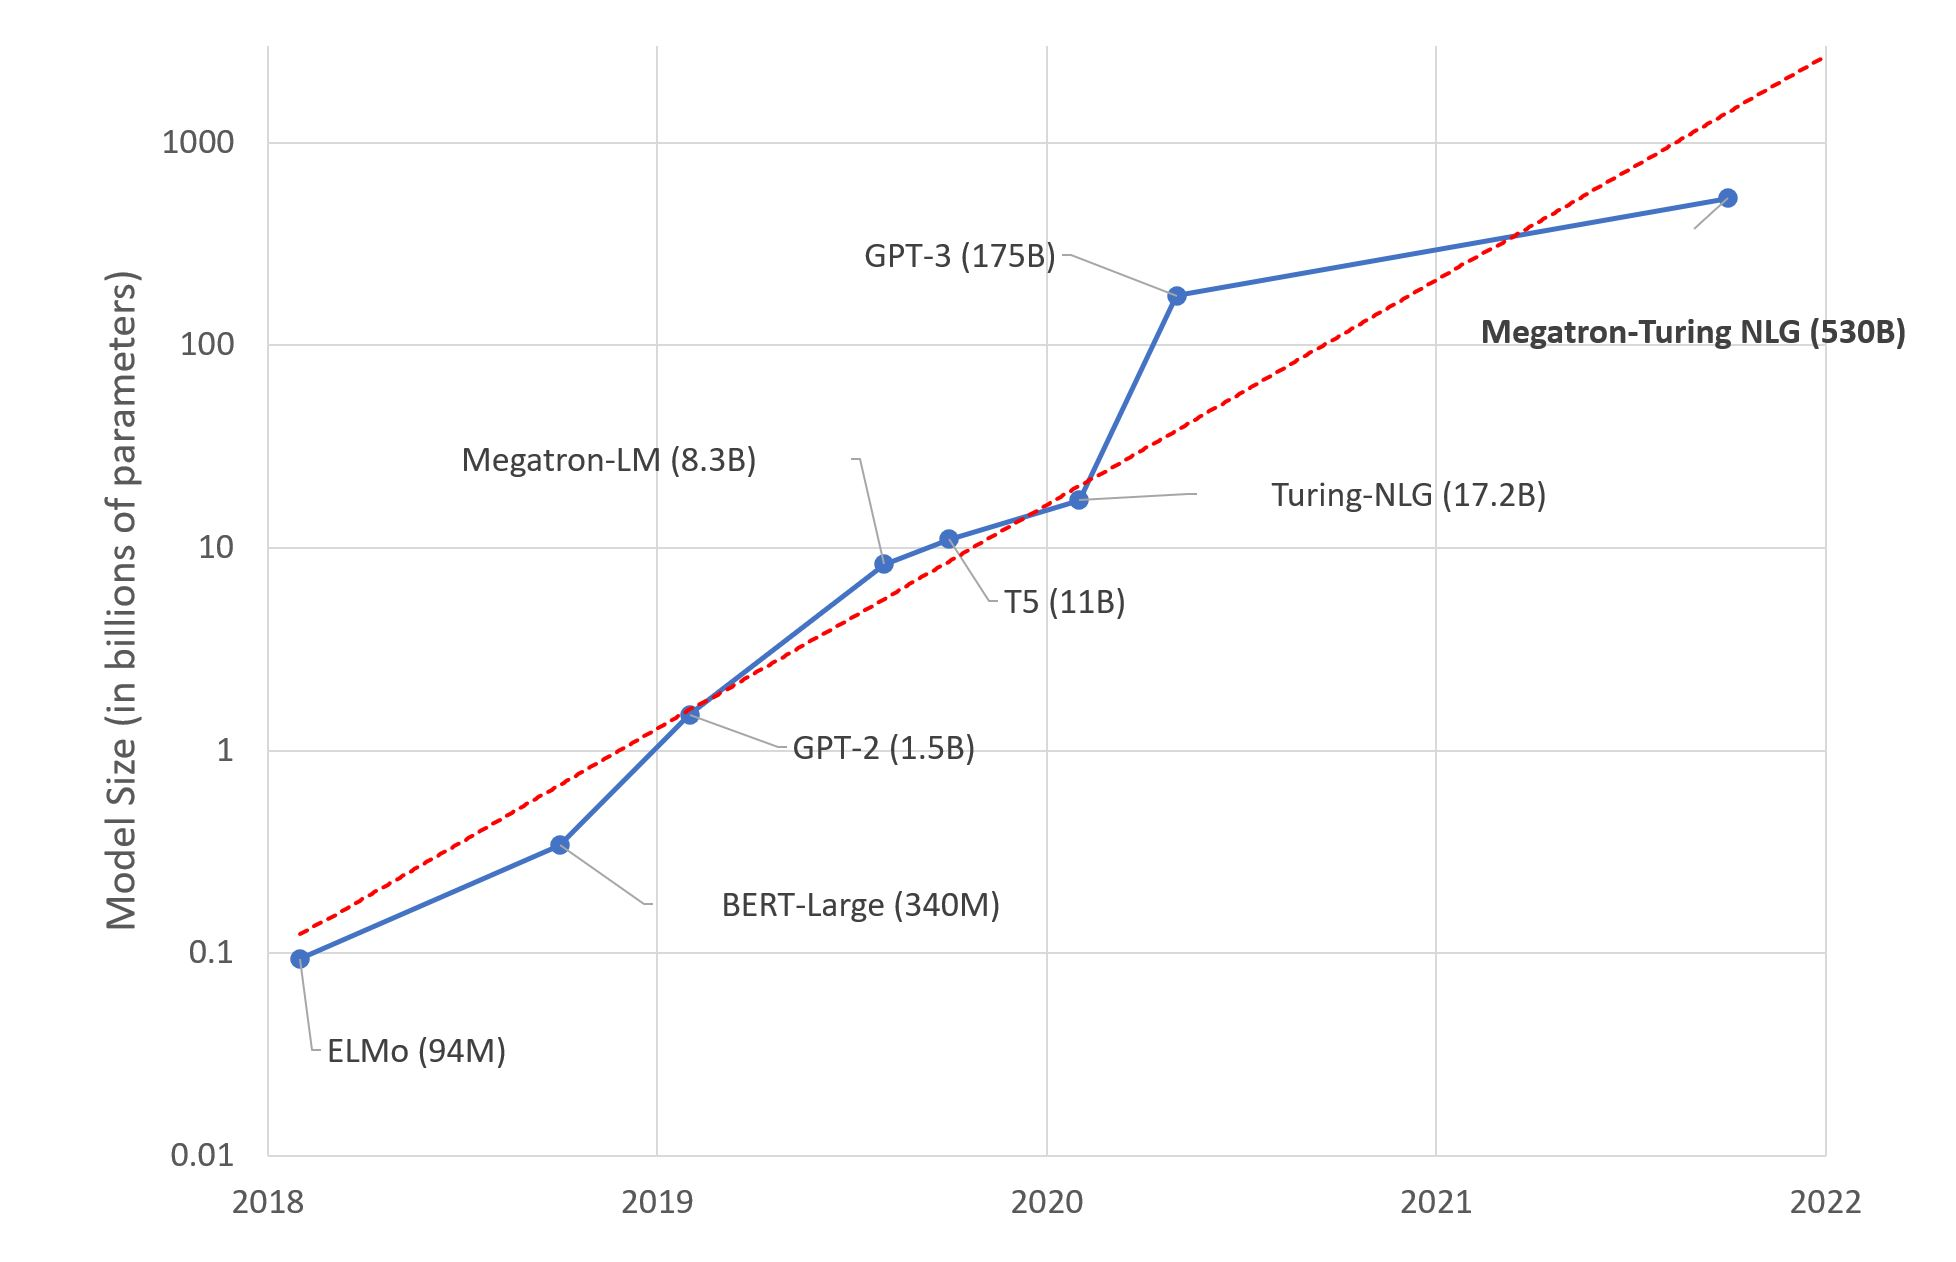
\includegraphics[width=\textwidth]{figs/model_sizes}
    \caption{Model Sizes (2018--2021)~\cite{model_sizes}}
    \label{fig:model_sizes}
\end{figure}

However, despite their state-of-the-art performance, the inner workings of these models are not yet fully understood and these models are still considered opaque or \emph{black-box}~\cite{lei-etal-2016-rationalizing}, which is a problem for their adoption in critical applications, such as healthcare or finance where decisions need to be explainable and interpretable.

Moreover, there is still a boundary to the capabilities of these models, regarding which problems can or cannot be solved by them and what can be learned and expressed by these models.

Strobl et.\ al\ \cite{strobl2024formal} defines two lines of work done regarding this problem: \textit{expressivity} and \textit{trainability}. This work will focus on the latter, as we aim to determine whether through training and using a \textit{white-box} approach, by looking at the attention mechanism and neural activations, whether Transformers are able to learn and classify sequences belonging to a formal language, more specifically, context-free grammars (CFGs) such as Dyck languages.

Chomsky's hierarchy\ \cite{chomsky-hierarchy} classifies CFGs as those languages that can be represented by a nondeterministic pushdown automaton, a class of automata that is more expressive than finite-state machines but less so than Turing machines~\cite{context-free-chomsky}. Pérez, Barceló and Marinkovic propose that architectures based on self-attention, such as Transformers, are Turing complete \cite{attention-tc}, therefore, this leads us to believe that CFGs can be expressed by these neural language models.

Based on the aforementioned, we seek to discuss whether attention patterns and neural activations in these architectures can be used to explain the model's classifications, and if these explanations can be leveraged to improve the model's performance and interpretability.

\bigskip

\textbf{Outline}

Chapter 2 will introduce the concepts behind formal languages and context-free grammars, focusing especially on the Chomsky Hierarchy and Dyck-$k$ languages.

Chapter 3 will introduce the Transformer architecture, with a focus towards the attention mechanism.

Chapter 4 will discuss related works and the state-of-the-art in the field of trainability of transformers, explainable AI and formal languages.

Chapter 5 focuses on the experimental setup, the dataset used, the model architecture, the training process and the obtained results.

Chapter 6 will discuss the results obtained and the implications of these results.

Chapter 7 will summarize the work done and propose future work.
